%%%%%%%%%%%%%%%%%%%%%%%%%%%%%%%%%%%%%%%%%%%%%%%%%%%%%%%%%%%%%%%%%
% Contents: The first start chapter
%%%%%%%%%%%%%%%%%%%%%%%%%%%%%%%%%%%%%%%%%%%%%%%%%%%%%%%%%%%%%%%%%

\chapter{Erster Start von Grisbi\label{start}}


\section{Assistent Basiskonfiguration\label{start-first}}

Nach der Installation von Grisbi wird Ihnen die Software beim ersten Start mit drei aufeinanderfolgenden Assistenten helfen:

\begin{enumerate}
	\item Der erste Assistent \dequote{Willkommen zu Grisbi}, der nur einmal, beim ersten Start, erscheint, hilft Ihnen bei der Konfiguration der Anwendung. Sie umfasst zwei Schritte, von denen der zweite die Verwaltung der \indexword{Kontodatei}\index{Kontodatei} betrifft (automatisches Laden und Speichern, Verschlüsselung und Sicherungskopien).%The first wizard \enquote{Welcome to Grisbi!}, which will only appear once, on first launch, helps you configure the application. It comprises two steps, the second of which concerns management of the \indexword{account file}\index{account file} (automatic loading and saving, encryption and backup copies).	
	
\begin{figure}[htbp]
	\begin{center}
		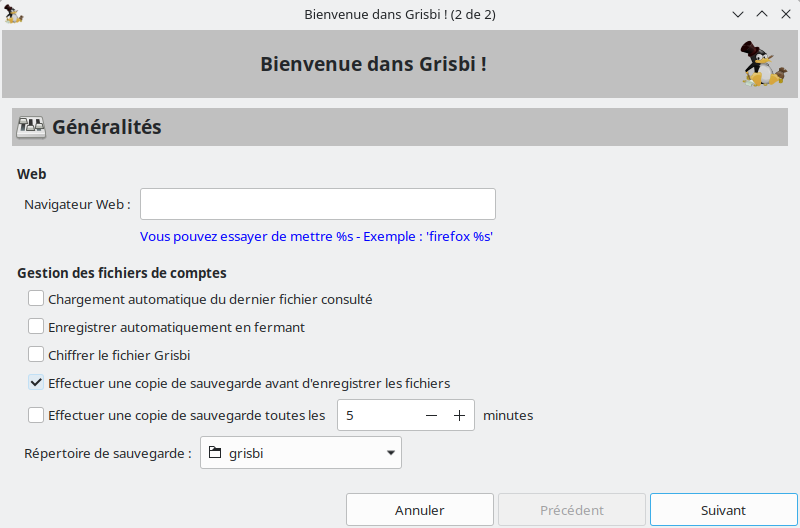
\includegraphics[width=.98\textwidth]{image/screenshot/start_first_launch}
	\end{center}
	\caption{Erstkonfiguration der Kontendatei.}
	\label{start_first_launch}
\end{figure}	
	
Es ist ratsam, die Optionen zu prüfen:%It is advisable to check the options:
	\begin{itemize}
		\item Die letzte Dateï automatisch öffnen;% Automatically load last file on startup%chargement automatique du dernier fichier consulté;
		\item Automatisch speichern;%Automatically save on exit;%enregistrer automatiquement en fermant;
		\item Vor dem Speichern eine Sicherung erstellen (standardmäßig aktiviert).%Make a backup copy before saving files (checked by default).%effectuer une copie de sauvegarde avant d'enregistrer les fichiers (coché par défaut).
	\end{itemize}
\end{enumerate}

\minisec{\Attention{}}
Die Grisbi-Entwickler empfehlen, die Option \menus{Datei verschlüsseln} aus den folgenden Gründen nicht zu verwenden:%The Grisbi developers recommend that you do not use the \menus{Encrypt Grisbi file} option for the following reasons:
\begin{itemize}
	\item Es gibt keine Methode zur Wiederherstellung einer verschlüsselten Datei, deren Passwort verloren gegangen ist;%there is no method for recovering an encrypted file whose password has been lost;
	\item Aus einem unbekannten Grund kann die Verwendung dieser Option unter Windows dazu führen, dass die Kontendatei völlig unbrauchbar wird.%For some unknown reason, using this option on Windows can render the accounts file completely unusable.
\end{itemize}  
Es ist jedoch ratsam, regelmäßig Sicherungskopien der unverschlüsselten Datei anzufertigen, wenn Sie sie verwenden.%However, if you use it, it is advisable to make regular back-ups of the unencrypted file.

\begin{enumerate}[resume]
	\item Der zweite Assistent, \dequote{Willkommen zu Grisbi} (oder später \dequote{Assistent für eine neue Datei}), der automatisch auf den ersten folgt, umfasst sechs Schritte, die Ihnen bei der Erstellung der \indexword{Kontodatei}\index{Kontodatei} helfen.%The second wizard, \dequote{Willkommen zu Grisbi} (or later \dequote{New file Assistant}), which automatically follows the first, includes six steps to help you create the \indexword{account file}\index{account file}.%Le deuxième assistant \frquote{Bienvenue dans Grisbi !} (ou plus tard \frquote{Aide à la création d'un nouveau fichier de comptes}), qui suit automatiquement le premier, comprend six étapes qui vous aiderons à la création du \indexword{fichier de comptes}\index{fichier de comptes}.
	\item Darauf folgt automatisch der dritte Assistent, \dequote{Ein neues Konto erstellen}, der zum Erstellen des ersten Kontos verwendet wird und im Abschnitt \ref{start-newfile} unten ausführlich beschrieben wird.%This is followed automatically by the third wizard, \dequote{Create a new account}, which is used to create the first account and is described in detail in section \ref{start-newfile} below.%Puis vient automatiquement le troisième assistant \frquote{Créer un nouveau compte} qui permet de créer le premier compte et qui est décrit en détail dans la section \ref{start-newfile} ci-dessous.
\end{enumerate}

Sie können jeden Assistenten jederzeit mit der Schaltfläche \menus{Abbrechen} verlassen.

Wenn Sie den Erststart-Assistenten nicht verwenden möchten, können Sie stattdessen eine Beispieldatei verwenden (siehe Abschnitt \ref{start-example} unten).

\section{Beispieldatei\label{start-example}}

Wenn Sie Grisbi sofort benutzen wollen, ohne die komplette Einrichtung durchlaufen zu müssen, zum Beispiel um eine Vorstellung von den Möglichkeiten dieses Programms zu bekommen, können Sie die Datei \file{Example\_3.0-de.gsb} von der \lang{Sourceforge.net}\footnote{\urlSourceForgeDocumentation{}} Website im Ordner \dequote{textsf{examples}} herunterladen.

\vspacepdf{5mm}
\Note{}: In dieser Beispieldatei sind die Namen der Zahlungsempfänger usw. reine Erfindung; jede Ähnlichkeit mit einer realen Person oder einem realen Unternehmen ist rein zufällig.%{Note}: in this example file, the names of the payees etc are pure invention; any similarity with a real person or business is entirely accidental.

\section{Erstellen einer neuen Kontodatei\label{start-newfile}}

Wenn Sie Grisbi zum ersten Mal verwenden, müssen Sie eine erste \indexword{Kontendatei}\index{Kontendatei} erstellen. Die \gls{Dateinamenserweiterung} lautet \file{.gsb} und der Dateiname \file{Name-ihrer-Datei.gsb}.%The \gls{extension} of this file will be \file{.gsb} and its name will be \file{your-file-name.gsb}.

Unmittelbar danach müssen Sie mindestens ein Konto (Bank-, Geld-, Passiv- oder Aktivkonto, beschrieben im Kapitel Kontoverwaltung) und einige weitere Konten (Giro-, Spar-, Kredit-, eventuell ein \vref{accounts} \menus{Verwaltung von Konten} und einige Übergangskonten) anlegen, die ihre jeweiligen Transaktionen enthalten werden.%Immediately afterwards, you will need to create at least one account (bank, cash, liability or asset account, described in the chapter \vref{accounts} \menus{Account management}), and then a few other accounts (current, savings, credit, possibly a cash account and a few transition accounts) which will contain their respective transactions.

Bei einer Familienverwaltung haben Sie normalerweise nur eine einzige Kontodatei, da dies den gesamten Austausch zwischen Ihren verschiedenen Konten ermöglicht. Wenn Sie einen Verein oder eine weitere Familie verwalten, die in keinem buchhalterischen Zusammenhang mit der ersten Familie steht, erstellen Sie eine weitere Kontodatei, die einen anderen Namen trägt \file{name-ihrer-zweiten-datei.gsb}. Dadurch bleiben die \indexword{Buchhaltungseinheiten}\index{Buchungsberechtigung} getrennt. %If you are managing a family, you will normally only have one accounts file, as this allows all the exchanges between your different accounts. If you are managing an association, or another family with no accounting relationship with the first, you will create another accounts file, which will have a different name your-second-file-name.gsb. This will keep the \indexword{accounting entities}\index{accounting entity} separate.

Mit anderen Worten: Alle Konten Ihres Haushalts werden in einer Kontendatei erfasst, alle Konten Ihrer Vereinigung in einer anderen Kontendatei.%In other words, all your household accounts are recorded in one file created by Grisbi, and all your association accounts are recorded in another file created by Grisbi.

\vspacepdf{5mm}

Das allgemeine Verfahren zur Erstellung einer Kontodatei ist wie folgt: Klicken Sie auf das \menus{Datei - Neue} oder auf die Schaltfläche Neu\refimage{start_grisbi}; der Assistent zur Erstellung einer Kontodatei wird geöffnet, der sechs Schritte umfasst, die im Folgenden beschrieben werden:

\begin{enumerate}
	\item Willkommensfenster (step 1/6): bestätigen Sie, indem Sie auf die Schaltfläche \menus{Nachfolgendes Element} klicken:%confirm by clicking on the \menus{Following} button:%validez par le bouton \menus{Suivant}:
	\item Allgemeine Konfiguration (Stufe 2/6)\refimage{start_file_create}:
	
	\begin{figure}[htbp]
		\begin{center}
			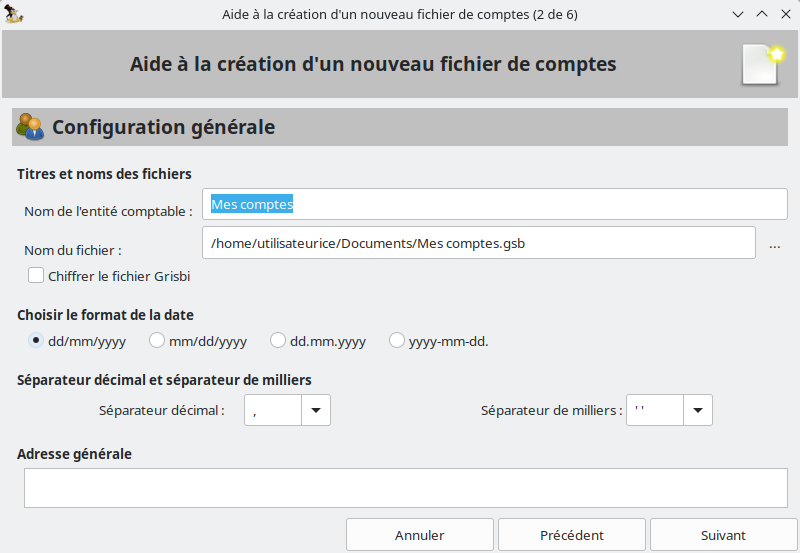
\includegraphics[width=0.98\textwidth]{image/screenshot/start_file_create}
		\end{center}
		\caption{Allgemeine Konfiguration einer Kontendatei}%General configuration of a accounts file}
		\label{start_file_create}
	\end{figure}

		\begin{enumerate}
			\item wählen Sie den Namen der Buchhaltungseinheit, deren Konten Sie verwalten, zum Beispiel \dequote{Meine Konten}, der als Titel der Startseite der Grisbi-Anwendung gewählt werden kann,%choose the name of the accounting entity whose accounts you manage, for example \enquote{My accounts}, which can be chosen as the title of the Grisbi application home page,%choisissez le nom de l'entité comptable dont vous gérez la comptabilité, par exemple \frquote{Ma comptabilité}, qui pourra être choisi comme titre de la page d'accueil de l'application Grisbi,
			\item Geben Sie den Namen der Kontendatei mit ihrer vollständigen Baumstruktur ein; standardmäßig schlägt Grisbi denselben Namen wie den der Buchhaltungseinheit vor, aber Sie können ihn ändern,%enter the name of the accounts file with its complete tree structure; by default, Grisbi suggests the same name as that of the accounting entity, but you can change it,%saisissez le nom du fichier de comptes avec son arborescence complète; Grisbi vous propose par défaut le même nom que celui de l'entité comptable, mais vous pouvez le 	modifier,
			\item aktivieren Sie das Kontrollkästchen \menus{Datei verschlüsseln}, wenn Sie die Kontodatei \gls{zu verschlüsseln} möchten,%check the \menus{Encrypt Grisbi} box if you wish \gls{to encrypt} the accounts file,%cochez la case \menus{Chiffrer le fichier Grisbi} si vous voulez \gls{chiffrer} le fichier de comptes,
		\end{enumerate}
		
\minisec{\Attention{}}
Die Entwickler von Grisbi empfehlen Ihnen aus den folgenden Gründen, die Option \menus{Datei verschlüsseln} nicht zu verwenden:%The Grisbi developers recommend that you do not use the \menus{Encrypt Grisbi file} option for the following reasons:
\begin{itemize}
	\item Es gibt keine Methode zur Wiederherstellung einer verschlüsselten Datei, deren Passwort verloren gegangen ist;%there is no method for recovering an encrypted file whose password has been lost;
	\item Aus einem unbekannten Grund kann die Verwendung dieser Option unter \gls{Windows} die Kontendatei völlig unbrauchbar machen.%For some unknown reason, using this option on Windows can render the accounts file completely unusable.
\end{itemize}  
Es ist jedoch ratsam, regelmäßig Sicherungskopien der unverschlüsselten Datei anzufertigen, wenn Sie sie verwenden.%However, if you use it, it is advisable to make regular back-ups of the unencrypted file.

		\begin{enumerate}[resume]		% to resume \end{enumerate} above \minisec
			\item wählen Sie das \indexword{Datumsformat}\index{Datumsformat} mit einer der vier Schaltflächen:%select the \indexword{date format}\index{date format} with one of the four buttons%sélectionnez le \indexword{format de la date}\index{format de date} avec l'un des quatre boutons:
			%\begin{addmargin}{-0.2cm}
				\begin{itemize}	
				\item[\textopenbullet] \dequote{dd/mm/yyyy} für \dequote{day/month/year},
				\item[\textopenbullet] \dequote{mm/dd/yyyy} für \dequote{month/day/year},
				\item[\textopenbullet] \dequote{dd.mm.yyyy} für \dequote{day.month.year},
				\item[\textopenbullet] \dequote{yyyy-mm-dd} für \dequote{year-month-day},
				\end{itemize}
			%\end{addmargin}
			\item wählen Sie das Dezimal \indexword{zeichen}\index{zeichen} und die Tausender aus den Dropdown-Listen,%choose the decimal \indexword{separator}\index{separator} and the thousands from the drop-down lists,%choisissez le \indexword{séparateur}\index{séparateur} décimal et celui des milliers dans les listes déroulantes,
			\item füllen Sie die Hauptadresse aus (optional)%fill in the address (optional),%renseignez l'adresse (facultatif),
			\item bestätigen Sie, indem Sie auf die Schaltfläche \menus{Nachfolgendes Element} klicken:%confirm with the  \menus{Following} button;%validez par le bouton \menus{Suivant};
		\end{enumerate}

	\item Auswahl der Basis\indexword{Währung}\index{Währung} (Stufe 3/6):%selection of the base \indexword{currency}\index{currency} (Stufe 3/6):%Sélection de la \indexword{devise}\index{devise} de base (étape 3/6):
		\begin{enumerate} 
		\item klicken Sie in der Liste auf die gewünschte Währung,%click on the chosen currency in the list,%cliquez sur la devise choisie dans la liste,
		\item Markieren Sie das Feld \dequote{Inklusive veralteter Währungen}, wenn Sie auch alte Währungen anzeigen möchten,%check the \enquote{Include obsolete currencies} box if you also want to display old currencies,%cochez la case \menus{Afficher les devises obsolètes} si vous voulez aussi afficher d'anciennes devises,
		\item bestätigen Sie, indem Sie auf die Schaltfläche \menus{Nachfolgendes Element} klicken:%confirm with the \menus{Following} button;%validez par le bouton \menus{Suivant};
		\end{enumerate}

	\item Auswahl des Indexwortes \indexword{Vordefinierte Kategorien}\index{Kategorien!Typen} (Stufe 4/6)\refimage{start_category_select}:%selection of the \indexword{list of categories}\index{catgories!types} you will use (step 4/6)\refimage{start_category_select}%sélection des \indexword{types de catégories}\index{catégories!types} utilisées (étape 4/6)\refimage{start_category_select}:
	
\begin{figure}[htbp]
	\begin{center}
		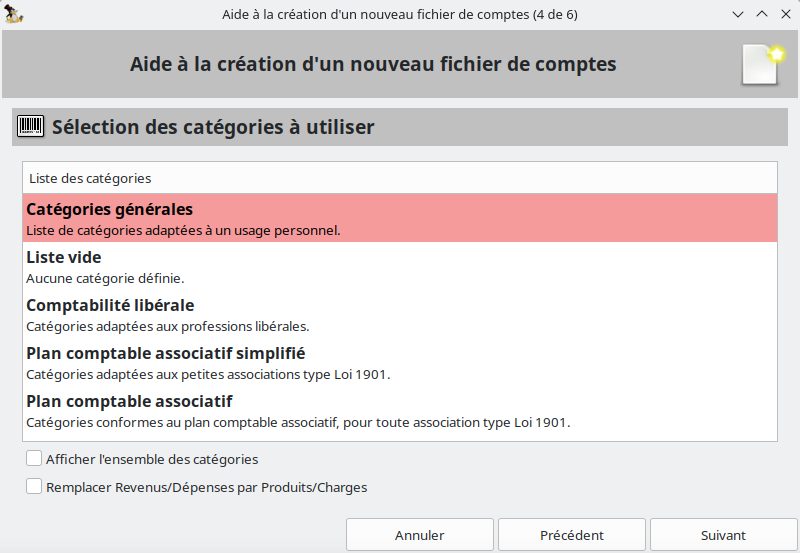
\includegraphics[width=0.98\textwidth]{image/screenshot/start_category_select}
	\end{center}
	\caption{Auswahl vordefinierter Kategorien}%Selection of categories to be used}%Sélection des catégories à utiliser}
\label{start_category_select}
\end{figure}

		\begin{enumerate} 
			\item klicken Sie auf die gewünschte Kategorie in der Liste;%cliquez sur la catégorie choisie dans la liste;
		%		 	\begin{itemize}
		%		 		\item\menus{Catégories générales},
		%		 		\item \menus{Liste vide},
		%		 		\item\menus{Comptabilité libérale},
		%		 		\item\menus{Plan comptable associatif simplifié}
		%		 		\item\menus{Plan comptable associatif},
		%		 	\end{itemize}
			\item aktivieren Sie das Kontrollkästchen \menus{Fremdkategorien anzeigen}, wenn Sie auch andere Kategorien mit englischem Namen anzeigen möchten,%cochez la case \menus{Afficher l'ensemble des catégories} si vous voulez aussi afficher d'autres catégories libellées en anglais,
			\item bestätigen Sie, indem Sie auf die Schaltfläche \menus{Nachfolgendes Element} klicken:%validez par le bouton \menus{Suivant};
		\end{enumerate}

	\item Geben Sie die Daten der \indexword{Banken}\index{Banken!Definition} ein, bei denen Ihre Konten geführt werden (Stufe 5/6):%Enter details of \indexword{banks}\index{banks!definition} holding your accounts (step 5/6):
		\begin{enumerate} 
			\item Klicken Sie auf \menus{Hinzufügen}, um eine Bank zu definieren; füllen Sie die Details der Bank aus (Name, Bankleitzahl usw.),%click \menus{Add} to define a bank; fill in the details of the bank (name, bank code, etc.),
			\item Wählen Sie eine Bank aus der Liste und klicken Sie auf die Schaltfläche \menus{Entfernen}, um eine Bank zu löschen, und bestätigen Sie dann im sich öffnenden Fenster,%select a bank from the list and click the \menus{Remove} button to delete a bank, then confirm in the window that opens,
			\item Bestätigen Sie mit der Schaltfläche \menus{Nachfolgendes Element}, um zum nächsten Schritt zu gelangen, \menus{Ein neues Konto erstellen}%Creating a new account}:%confirm with the \menus{Forward} button to go to the next step, \menus{Creating a new account}:
		\end{enumerate} 

	\item Konfiguration beendet (Stufe 6/6):\par%Configuration finished (step 6/6):\par
	Die Konfiguration der Kontendatei ist nun abgeschlossen, und im folgenden Fenster werden Sie aufgefordert, eine der beiden Methoden für die Erstellung Ihres ersten Kontos zu wählen\refimage{start_account_choice}:%The configuration of the accounts file is now complete, and the window below will ask you to choose one of the two methods for creating your first account\refimage{start_account_choice}:

\vspace{2mm}

\begin{figure}[htbp]
	\begin{center}
		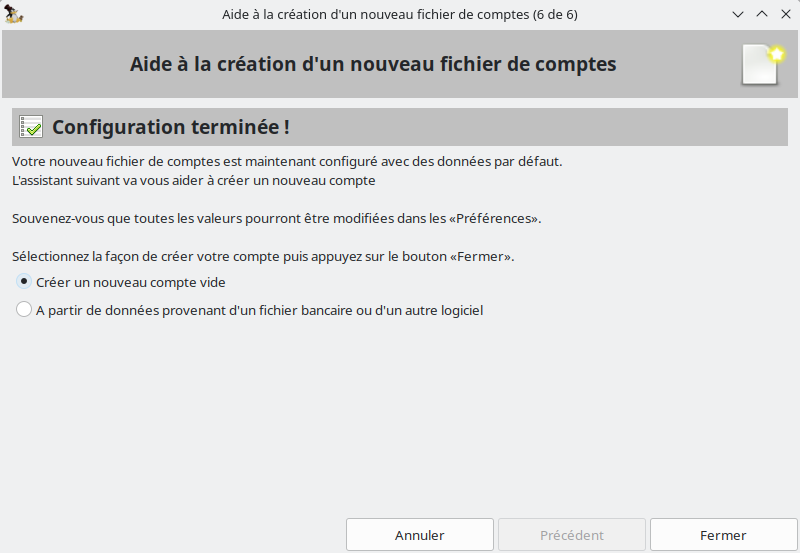
\includegraphics[width=0.98\textwidth]{image/screenshot/start_account_choice}
	\end{center}
	\caption{Auswahlmöglichkeiten bei der Erstellung Ihres ersten Kontos}
	\label{start_account_choice}
\end{figure}

	\begin{itemize}
		\item[\textopenbullet] \menus{Ein neues Konto manuell erstellen}:\par%Create a new account from scratch}:\par
		Wenn Sie diese Zeile ankreuzen und dann mit der Schaltfläche \menus{Schließen} bestätigen, wird dieses Fenster geschlossen und der Assistent \dequote{Ein neues Konto erstellen} gestartet. Siehe \vref{accounts-new}, \menus{Erstellen eines neuen Kontos}, wo dieses Verfahren ausführlich beschrieben wird, und kehren Sie dann zu dieser Seite zurück;%If you check this line, then if you confirm with the \menus{Close} button, this window closes and the \enquote{Create a new account} wizard starts. See \vref{accounts-new}, \menus{Creating a new account}, which fully describes this procedure, then return to this page;
	
		\item[\textopenbullet] \menus{Konten und Daten von anderen Finanzprogrammen oder Ihrer Bank importieren}:\par%Import data from online bank services or from accounting software}:\par
		Wenn Sie diese Zeile ankreuzen und dann mit der Schaltfläche \menus{Schließen} bestätigen, wird dieses Fenster geschlossen und der \dequote{Daten importieren} Assistent zum Importieren von Daten aus einer Buchhaltungsdatei, startet. Siehe den Abschnitt \vref{move-import-importinit}, \menus{Importieren von Kontendateien aus einem anderen Programm in Grisbi}, in dem dieses Verfahren ausführlich beschrieben wird, und kehren Sie dann zu dieser Seite zurück.%If you check this line and then confirm with the \menus{Close} button, this window closes and the \enquote{New file Assistant to import} Wizard for importing data from an accounts file, starts. See the \vref{move-import-importinit} section, \menus{Importing Account Files from Another Programme into Grisbi}, which fully describes this procedure, then return to this page.
	\end{itemize}
\end{enumerate}

\label{start-newfile-end}

\textit{\textbf{Auf die eine oder andere Weise}} haben Sie nun Ihre Grisbi-Datei sowie das erste Konto für diese Datei erstellt.%{In one way or another}}, you have now created your Grisbi file, as well as the first account of this file.

\vspacepdf{5mm}

Wenn Sie jetzt weitere Konten erstellen möchten, wählen Sie das Menü {Bearbeiten - Konto erstellen}, um ein weiteres Konto zu erstellen (siehe den Abschnitt \vref{accounts-new}, \menus{Ein neues Konto erstellen}).%If you want to create other accounts now, select the \menus{Edit - New Account} to create another account (see the \vref{accounts-new}, \menus{Creating a new account} section).

\vspacepdf{5mm}

Andernfalls können Sie das soeben erstellte Konto oder das Konto, von dem Sie die Daten gerade importiert haben, verwenden.%Otherwise, you can start using the account you just created or the one from which you just imported the data.

\minisec{\Attention{}}%Warning
Im Allgemeinen ist es nicht ratsam, Akzente oder Leerzeichen in den Namen der von Grisbi verwendeten Verzeichnisse und Dateien zu verwenden. Wenn dies der Fall ist, benennen Sie sie jetzt um. Leerzeichen können beispielsweise durch Unterstriche (\underline{}) ersetzt werden.%In general, it is inadvisable to have accents or spaces in the names of directories and files used by Grisbi. If so, rename them now. For example, spaces can be replaced by underscores (\underline{}).

\section{Speichern Ihrer Kontendatei\label{start-save}}%Saving your accounts file\label{start-save}}

Ihre Operationen werden nicht wie bei anderen Programmen direkt bei der Eingabe geschrieben, sondern Sie müssen Ihre Kontodatei vor dem Beenden speichern. Keine Sorge, Grisbi warnt Sie, wenn Sie dies nicht getan haben.%Your operations are not written as you enter them as they might be in other software; you must therefore save your account file before exiting. Do not worry, Grisbi warns you if you have not done so.

Sie können die Optionen zum Speichern der Kontodatei im Menü \menus{Bearbeiten - Einstellungen} konfigurieren, siehe den Abschnitt \vref{setup-general-files-manage}, \menus{Verwaltung von Kontodateien}%Managing Account Files}.%You can configure the options for saving the account file in the \menus{Edit - Preferences} menu, see the section \vref{setup-general-files-manage}, \menus{Managing Account Files}.


\section{Import aus anderen Buchhaltungssystemen}%Import from other personal accounting software}

Siehe den Abschnitt \vref{move-import-importinit}, um Kontodateien aus einem anderen Programm in Grisbi zu importieren. Im Moment unterstützt Grisbi die Formate \gls{Gnucash}, \gls{OFX}, \GLS{CSV} und \GLS{QIF}.%See the \vref{move-import-importinit} section to import account files from another program into Grisbi. For the moment, Grisbi supports \gls{Gnucash}, \gls{OFX}, \GLS{CSV} and \GLS{QIF} formats.